
%%%%%%%%%%%%%%%%%% PREAMBULE %%%%%%%%%%%%%%%%%%

\documentclass[aspectratio=169,utf8]{beamer}
%\documentclass[aspectratio=169,handout]{beamer}

\usetheme{Boadilla}
%\usecolortheme{seahorse}
\usecolortheme[RGB={245,66,24}]{structure}
\useoutertheme{infolines}

% packages
\usepackage{amsfonts,amsmath,amssymb,amsthm}
\usepackage[utf8]{inputenc}
\usepackage[T1]{fontenc}
\usepackage{lmodern}

\usepackage[francais]{babel}
\usepackage{fancybox}
\usepackage{graphicx}

\usepackage{float}
\usepackage{xfrac}

%\usepackage[usenames, x11names]{xcolor}
\usepackage{tikz}
\usepackage{pgfplots}
\usepackage{datetime}



%-----  Package unités -----
\usepackage{siunitx}
\sisetup{locale = FR,detect-all,per-mode = symbol}

%\usepackage{mathptmx}
%\usepackage{fouriernc}
%\usepackage{newcent}
%\usepackage[mathcal,mathbf]{euler}

%\usepackage{palatino}
%\usepackage{newcent}
% \usepackage[mathcal,mathbf]{euler}



% \usepackage{hyperref}
% \hypersetup{colorlinks=true, linkcolor=blue, urlcolor=blue,
% pdftitle={Exo7 - Exercices de mathématiques}, pdfauthor={Exo7}}


%section
% \usepackage{sectsty}
% \allsectionsfont{\bf}
%\sectionfont{\color{Tomato3}\upshape\selectfont}
%\subsectionfont{\color{Tomato4}\upshape\selectfont}

%----- Ensembles : entiers, reels, complexes -----
\newcommand{\Nn}{\mathbb{N}} \newcommand{\N}{\mathbb{N}}
\newcommand{\Zz}{\mathbb{Z}} \newcommand{\Z}{\mathbb{Z}}
\newcommand{\Qq}{\mathbb{Q}} \newcommand{\Q}{\mathbb{Q}}
\newcommand{\Rr}{\mathbb{R}} \newcommand{\R}{\mathbb{R}}
\newcommand{\Cc}{\mathbb{C}} 
\newcommand{\Kk}{\mathbb{K}} \newcommand{\K}{\mathbb{K}}

%----- Modifications de symboles -----
\renewcommand{\epsilon}{\varepsilon}
\renewcommand{\Re}{\mathop{\text{Re}}\nolimits}
\renewcommand{\Im}{\mathop{\text{Im}}\nolimits}
%\newcommand{\llbracket}{\left[\kern-0.15em\left[}
%\newcommand{\rrbracket}{\right]\kern-0.15em\right]}

\renewcommand{\ge}{\geqslant}
\renewcommand{\geq}{\geqslant}
\renewcommand{\le}{\leqslant}
\renewcommand{\leq}{\leqslant}
\renewcommand{\epsilon}{\varepsilon}

%----- Fonctions usuelles -----
\newcommand{\ch}{\mathop{\text{ch}}\nolimits}
\newcommand{\sh}{\mathop{\text{sh}}\nolimits}
\renewcommand{\tanh}{\mathop{\text{th}}\nolimits}
\newcommand{\cotan}{\mathop{\text{cotan}}\nolimits}
\newcommand{\Arcsin}{\mathop{\text{arcsin}}\nolimits}
\newcommand{\Arccos}{\mathop{\text{arccos}}\nolimits}
\newcommand{\Arctan}{\mathop{\text{arctan}}\nolimits}
\newcommand{\Argsh}{\mathop{\text{argsh}}\nolimits}
\newcommand{\Argch}{\mathop{\text{argch}}\nolimits}
\newcommand{\Argth}{\mathop{\text{argth}}\nolimits}
\newcommand{\pgcd}{\mathop{\text{pgcd}}\nolimits} 


%----- Commandes divers ------
\newcommand{\ii}{\mathrm{i}}
\newcommand{\dd}{\text{d}}
\newcommand{\id}{\mathop{\text{id}}\nolimits}
\newcommand{\Ker}{\mathop{\text{Ker}}\nolimits}
\newcommand{\Card}{\mathop{\text{Card}}\nolimits}
\newcommand{\Vect}{\mathop{\text{Vect}}\nolimits}
\newcommand{\Mat}{\mathop{\text{Mat}}\nolimits}
\newcommand{\rg}{\mathop{\text{rg}}\nolimits}
\newcommand{\tr}{\mathop{\text{tr}}\nolimits}


%----- Structure des exercices ------

\newtheoremstyle{styleexo}% name
{2ex}% Space above
{3ex}% Space below
{}% Body font
{}% Indent amount 1
{\bfseries} % Theorem head font
{}% Punctuation after theorem head
{\newline}% Space after theorem head 2
{}% Theorem head spec (can be left empty, meaning ‘normal’)

%\theoremstyle{styleexo}
\newtheorem{exo}{Exercice}
\newtheorem{ind}{Indications}
\newtheorem{cor}{Correction}


\newcommand{\exercice}[1]{} \newcommand{\finexercice}{}
%\newcommand{\exercice}[1]{{\tiny\texttt{#1}}\vspace{-2ex}} % pour afficher le numero absolu, l'auteur...
\newcommand{\enonce}{\begin{exo}} \newcommand{\finenonce}{\end{exo}}
\newcommand{\indication}{\begin{ind}} \newcommand{\finindication}{\end{ind}}
\newcommand{\correction}{\begin{cor}} \newcommand{\fincorrection}{\end{cor}}

\newcommand{\noindication}{\stepcounter{ind}}
\newcommand{\nocorrection}{\stepcounter{cor}}

\newcommand{\fiche}[1]{} \newcommand{\finfiche}{}
\newcommand{\titre}[1]{\centerline{\large \bf #1}}
\newcommand{\addcommand}[1]{}
\newcommand{\video}[1]{}

% Marge
\newcommand{\mymargin}[1]{\marginpar{{\small #1}}}

\def\noqed{\renewcommand{\qedsymbol}{}}


%----- Presentation ------
\setlength{\parindent}{0cm}

%\newcommand{\ExoSept}{\href{http://exo7.emath.fr}{\textbf{\textsf{Exo7}}}}

\definecolor{myred}{rgb}{0.93,0.26,0}
\definecolor{myorange}{rgb}{0.97,0.58,0}
\definecolor{myyellow}{rgb}{1,0.86,0}

\newcommand{\LogoExoSept}[1]{  % input : echelle
{\usefont{U}{cmss}{bx}{n}
\begin{tikzpicture}[scale=0.1*#1,transform shape]
  \fill[color=myorange] (0,0)--(4,0)--(4,-4)--(0,-4)--cycle;
  \fill[color=myred] (0,0)--(0,3)--(-3,3)--(-3,0)--cycle;
  \fill[color=myyellow] (4,0)--(7,4)--(3,7)--(0,3)--cycle;
  \node[scale=5] at (3.5,3.5) {Exo7};
\end{tikzpicture}}
}


\newcommand{\debutmontitre}{
  \author{} \date{} 
  \thispagestyle{empty}
  \hspace*{-10ex}
  \begin{minipage}{\textwidth}
    \titlepage  
  \vspace*{-2.5cm}
  \begin{center}
    \LogoExoSept{2.5}
  \end{center}
  \end{minipage}

  \vspace*{-0cm}
  
  % Astuce pour que le background ne soit pas discrétisé lors de la conversion pdf -> png
\begin{tikzpicture}
        \fill[opacity=0,green!60!black] (0,0)--++(0,0)--++(0,0)--++(0,0)--cycle; 
\end{tikzpicture}

% toc S'affiche trop tot :
% \tableofcontents[hideallsubsections, pausesections]
}

\newcommand{\finmontitre}{
  \end{frame}
  \setcounter{framenumber}{0}
} % ne marche pas pour une raison obscure

%----- Commandes supplementaires ------

% \usepackage[landscape]{geometry}
% \geometry{top=1cm, bottom=3cm, left=2cm, right=10cm, marginparsep=1cm
% }
% \usepackage[a4paper]{geometry}
% \geometry{top=2cm, bottom=2cm, left=2cm, right=2cm, marginparsep=1cm
% }

%\usepackage{standalone}


% New command Arnaud -- november 2011
\setbeamersize{text margin left=24ex}
% si vous modifier cette valeur il faut aussi
% modifier le decalage du titre pour compenser
% (ex : ici =+10ex, titre =-5ex

\theoremstyle{definition}
%\newtheorem{proposition}{Proposition}
%\newtheorem{exemple}{Exemple}
%\newtheorem{theoreme}{Théorème}
%\newtheorem{lemme}{Lemme}
%\newtheorem{corollaire}{Corollaire}
%\newtheorem*{remarque*}{Remarque}
%\newtheorem*{miniexercice}{Mini-exercices}
%\newtheorem{definition}{Définition}

% Commande tikz
\usetikzlibrary{calc}
\usetikzlibrary{patterns,arrows}
\usetikzlibrary{matrix}
\usetikzlibrary{fadings} 

%definition d'un terme
\newcommand{\defi}[1]{{\color{myorange}\textbf{\emph{#1}}}}
\newcommand{\evidence}[1]{{\color{blue}\textbf{\emph{#1}}}}
\newcommand{\assertion}[1]{\emph{\og#1\fg}}  % pour chapitre logique
%\renewcommand{\contentsname}{Sommaire}
\renewcommand{\contentsname}{}
\setcounter{tocdepth}{2}



%------ Figures ------

\def\myscale{1} % par défaut 
\newcommand{\myfigure}[2]{  % entrée : echelle, fichier figure
\def\myscale{#1}
\begin{center}
\footnotesize
{#2}
\end{center}}


%------ Encadrement ------

\usepackage{fancybox}


\newcommand{\mybox}[1]{
\setlength{\fboxsep}{7pt}
\begin{center}
\shadowbox{#1}
\end{center}}

\newcommand{\myboxinline}[1]{
\setlength{\fboxsep}{5pt}
\raisebox{-10pt}{
\shadowbox{#1}
}
}

%--------------- Commande beamer---------------
\newcommand{\beameronly}[1]{#1} % permet de mettre des pause dans beamer pas dans poly


\setbeamertemplate{navigation symbols}{}
\setbeamertemplate{footline}  % tiré du fichier beamerouterinfolines.sty
{
  \leavevmode%
  \hbox{%
  \begin{beamercolorbox}[wd=.333333\paperwidth,ht=2.25ex,dp=1ex,center]{author in head/foot}%
    % \usebeamerfont{author in head/foot}\insertshortauthor%~~(\insertshortinstitute)
    \usebeamerfont{section in head/foot}{\bf\insertshorttitle}
  \end{beamercolorbox}%
  \begin{beamercolorbox}[wd=.333333\paperwidth,ht=2.25ex,dp=1ex,center]{title in head/foot}%
    \usebeamerfont{section in head/foot}{\bf\insertsectionhead}
  \end{beamercolorbox}%
  \begin{beamercolorbox}[wd=.333333\paperwidth,ht=2.25ex,dp=1ex,right]{date in head/foot}%
    % \usebeamerfont{date in head/foot}\insertshortdate{}\hspace*{2em}
    \insertframenumber{} / \inserttotalframenumber\hspace*{2ex} 
  \end{beamercolorbox}}%
  \vskip0pt%
}


\definecolor{mygrey}{rgb}{0.5,0.5,0.5}
\setlength{\parindent}{0cm}
%\DeclareTextFontCommand{\helvetica}{\fontfamily{phv}\selectfont}

% background beamer
\definecolor{couleurhaut}{rgb}{0.85,0.9,1}  % creme
\definecolor{couleurmilieu}{rgb}{1,1,1}  % vert pale
\definecolor{couleurbas}{rgb}{0.85,0.9,1}  % blanc
\setbeamertemplate{background canvas}[vertical shading]%
[top=couleurhaut,middle=couleurmilieu,midpoint=0.4,bottom=couleurbas] 
%[top=fondtitre!05,bottom=fondtitre!60]



\makeatletter
\setbeamertemplate{theorem begin}
{%
  \begin{\inserttheoremblockenv}
  {%
    \inserttheoremheadfont
    \inserttheoremname
    \inserttheoremnumber
    \ifx\inserttheoremaddition\@empty\else\ (\inserttheoremaddition)\fi%
    \inserttheorempunctuation
  }%
}
\setbeamertemplate{theorem end}{\end{\inserttheoremblockenv}}

\newenvironment{theoreme}[1][]{%
   \setbeamercolor{block title}{fg=structure,bg=structure!40}
   \setbeamercolor{block body}{fg=black,bg=structure!10}
   \begin{block}{{\bf Th\'eor\`eme }#1}
}{%
   \end{block}%
}


\newenvironment{proposition}[1][]{%
   \setbeamercolor{block title}{fg=structure,bg=structure!40}
   \setbeamercolor{block body}{fg=black,bg=structure!10}
   \begin{block}{{\bf Proposition }#1}
}{%
   \end{block}%
}

\newenvironment{corollaire}[1][]{%
   \setbeamercolor{block title}{fg=structure,bg=structure!40}
   \setbeamercolor{block body}{fg=black,bg=structure!10}
   \begin{block}{{\bf Corollaire }#1}
}{%
   \end{block}%
}

\newenvironment{mydefinition}[1][]{%
   \setbeamercolor{block title}{fg=structure,bg=structure!40}
   \setbeamercolor{block body}{fg=black,bg=structure!10}
   \begin{block}{{\bf Définition} #1}
}{%
   \end{block}%
}

\newenvironment{lemme}[0]{%
   \setbeamercolor{block title}{fg=structure,bg=structure!40}
   \setbeamercolor{block body}{fg=black,bg=structure!10}
   \begin{block}{\bf Lemme}
}{%
   \end{block}%
}

\newenvironment{remarque}[1][]{%
   \setbeamercolor{block title}{fg=black,bg=structure!20}
   \setbeamercolor{block body}{fg=black,bg=structure!5}
   \begin{block}{Remarque #1}
}{%
   \end{block}%
}


\newenvironment{exemple}[1][]{%
   \setbeamercolor{block title}{fg=black,bg=structure!20}
   \setbeamercolor{block body}{fg=black,bg=structure!5}
   \begin{block}{{\bf Exemple }#1}
}{%
   \end{block}%
}


\newenvironment{miniexercice}[0]{%
   \setbeamercolor{block title}{fg=structure,bg=structure!20}
   \setbeamercolor{block body}{fg=black,bg=structure!5}
   \begin{block}{Mini-exercices}
}{%
   \end{block}%
}


\newenvironment{tp}[0]{%
   \setbeamercolor{block title}{fg=structure,bg=structure!40}
   \setbeamercolor{block body}{fg=black,bg=structure!10}
   \begin{block}{\bf Travaux pratiques}
}{%
   \end{block}%
}
\newenvironment{exercicecours}[1][]{%
   \setbeamercolor{block title}{fg=structure,bg=structure!40}
   \setbeamercolor{block body}{fg=black,bg=structure!10}
   \begin{block}{{\bf Exercice }#1}
}{%
   \end{block}%
}
\newenvironment{algo}[1][]{%
   \setbeamercolor{block title}{fg=structure,bg=structure!40}
   \setbeamercolor{block body}{fg=black,bg=structure!10}
   \begin{block}{{\bf Algorithme}\hfill{\color{gray}\texttt{#1}}}
}{%
   \end{block}%
}


\setbeamertemplate{proof begin}{
   \setbeamercolor{block title}{fg=black,bg=structure!20}
   \setbeamercolor{block body}{fg=black,bg=structure!5}
   \begin{block}{{\footnotesize Démonstration}}
   \footnotesize
   \smallskip}
\setbeamertemplate{proof end}{%
   \end{block}}
\setbeamertemplate{qed symbol}{\openbox}


\makeatother
\usecolortheme[RGB={127,0,0}]{structure}

% Commande spécifique à ce chapitre

\newcommand{\Python}{\texttt{Python}}
\renewcommand{\evidence}[1]{{\color{blue}\textbf{#1}}}

\usepackage{textcomp}

\usepackage{listings}
\lstset{
  upquote=true,
  columns=flexible,
  keepspaces=true,
  basicstyle=\ttfamily,
  commentstyle=\color{gray},
  language=Python,
  showstringspaces=false,
  aboveskip=0em,  
  belowskip=0em,
  escapeinside=||
}

\lstset{
  literate={é}{{\'e}}1
           {è}{{\`e}}1
           {à}{{\`a}}1
}


\newcommand{\codeinline}[1]{\lstinline!#1!}


\definecolor{coul_prive}{rgb}{0.93,0.26,0}
\definecolor{coul_public}{rgb}{0.06,0.63,0}

\newcommand{\prive}[1]{{\color{coul_prive} #1}}
\newcommand{\public}[1]{{\color{coul_public} #1}}


% Boites pour les exemples
\newenvironment{exempleun}{%
   \setbeamercolor{block title}{fg=structure,bg=structure!40}
   \setbeamercolor{block body}{fg=black,bg=structure!10}
   \begin{block}{\hfill{\small \color{black}{\bf Exemple facile}}}
}{%
   \end{block}%
}

\newenvironment{exempledeux}{%
   \setbeamercolor{block title}{fg=structure,bg=structure!60}
   \setbeamercolor{block body}{fg=black,bg=structure!20}
   \begin{block}{\hfill{\small \color{black}{\bf Exemple dur}}}
}{%
   \end{block}%
}
 
%%%%%%%%%%%%%%%%%%%%%%%%%%%%%%%%%%%%%%%%%%%%%%%%%%%%%%%%%%%%%
%%%%%%%%%%%%%%%%%%%%%%%%%%%%%%%%%%%%%%%%%%%%%%%%%%%%%%%%%%%%%


\begin{document}


\title{{\bf Cryptographie}}
\subtitle{Le chiffrement RSA}

\begin{frame}
  
  \debutmontitre

  \pause

{\footnotesize
\hfill
\setbeamercovered{transparent=50}
\begin{minipage}{0.6\textwidth}
  \begin{itemize}
    \item<3-> Calcul de la clé publique et de la clé privée
    \item<4-> Chiffrement du message
    \item<5-> Déchiffrement du message
    \item<6-> Algorithmes
  \end{itemize}
\end{minipage}
}

\end{frame}

\setcounter{framenumber}{0}


%%%%%%%%%%%%%%%%%%%%%%%%%%%%%%%%%%%%%%%%%%%%%%%%%%%%%%%%%%%%%%%%
\section{Le chiffrement RSA}

\begin{frame}


\begin{itemize}
  \item Problème difficile : 

factoriser un entier produit de deux \evidence{nombres premiers distincts} 
\pause
  \item Clé publique et clé secrète  :

calculées à l'aide de l'\evidence{algorithme d'Euclide} 
et des \evidence{coefficients de Bézout}
\pause
  \item Environnement :

calculs \evidence{modulo} un entier
\pause
  \item Déchiffrement :

fonctionne grâce au \evidence{petit théorème de Fermat}
\end{itemize}

\bigskip
\pause

Bruno veut envoyer un message secret à Alice
\pause
\begin{enumerate}
  \item Alice prépare une clé publique et une clé privée
\pause  
  \item Bruno utilise la clé publique d'Alice pour crypter son message
\pause  
  \item Alice reçoit le message crypté et le déchiffre grâce à sa clé privée
\end{enumerate}
\end{frame}


%%%%%%%%%%%%%%%%%%%%%%%%%%%%%%%%%%%%%%%%%%%%%%%%%%%%%%%%%%%%%%%%
\section{Calcul de la clé publique et de la clé privée}

\begin{frame}[fragile]

\evidence{\'Etape 1. Préparation des clés}

\pause

\evidence{\'Etape 1.1 Choix de deux nombres premiers}

Alice effectue les opérations suivantes
\begin{itemize}
  \item choix de deux nombres premiers distincts $\prive{p}$ et $\prive{q}$
  
  \item calcul de $\public{n} = \prive{p} \times \prive{q}$
  
  \item calcul de $\varphi(\public{n}) = (\prive{p}-1) \times (\prive{q}-1)\ = \prive{\varphi(n)} $
\end{itemize}

\pause

\begin{exempleun}
 \begin{itemize}
  \item $\prive{p} = 5$ et $\prive{q} = 17$ 
  
  \item $\public{n} = \prive{p} \times \prive{q} = 85$
  
  \item $\varphi(\public{n}) = (\prive{p}-1) \times (\prive{q}-1) = \prive{\varphi(n)} = 64$
\end{itemize}   
\end{exempleun}

%% \pause

%% \begin{exempledeux}
%%  \begin{itemize}
%%   \item $\prive{p} = 101$ et $\prive{q} = 103$ 
  
%%   \item $\public{n} = \prive{p} \times \prive{q} = 10\;403$
  
%%   \item $\varphi(\public{n}) = (\prive{p}-1) \times (\prive{q}-1) = \prive{\varphi(n)} = 10\;200$
%% \end{itemize}   
%% \end{exempledeux}

\end{frame}

\begin{frame}

\evidence{\'Etape 1. Préparation des clés}

\evidence{\'Etape 1.2 Choix d'un exposant et calcul de son inverse}

\pause

\begin{itemize}
  \item Alice choisit un exposant $\public{e}$ tel que $\pgcd(\public{e},\prive{\varphi(n)})=1$

\pause

  \item Alice calcule l'inverse $\prive{d}$ de $\public{e}$ module $\prive{\varphi(n)}$ par l'algorithme d'Euclide étendu 
  :  $\prive{d} \times \public{e} \equiv 1 \pmod {\prive{\varphi(n)}}$
\end{itemize}

\bigskip
\pause

\begin{exempleun}
\begin{itemize}
  \item $\public{e} = 5$ et on a bien  $\pgcd(\public{e},\prive{\varphi(n)}) = \pgcd(5,64)=1$
\pause  
  \item 
  \begin{itemize}
    \item $5 \times 13 + 64 \times (-1) = 1$
    \item donc $5 \times 13 \equiv 1 \pmod {64}$
    \item l'inverse de $\public{e}$ modulo $\prive{\varphi(n)}$ est $\prive{d} = 13$
  \end{itemize}
  
  
\end{itemize}  
\end{exempleun}
%% \pause

%% \begin{exempledeux}
%% \begin{itemize}
%%   \item $\public{e} = 7$ et on bien  $\pgcd(\public{e},\prive{\varphi(n)})= \pgcd(7,10\;200)=1$
%% \pause  
%%   \item
%%   \begin{itemize}
%%     \item $7 \times (-1457) + 10\; 200 \times 1 = 1$
%%     \item mais $-1457 \equiv 8743\pmod{\prive{\varphi(n)}}$
%%     \item donc $\prive{d} = 8743 $
%%   \end{itemize}
%% \end{itemize}  
%% \end{exempledeux}


\end{frame}





\begin{frame}

\evidence{\'Etape 1. Préparation des clés}

\evidence{\'Etape 1.3 Clé publique}

La \defi{clé publique} d'Alice est constituée des deux nombres 
\mybox{$\public{n}$ \  et \  $\public{e}$}

\pause

\evidence{\'Etape 1.4 Clé privée}

Alice garde pour elle sa \defi{clé privée} 
\mybox{\ $\prive{d}$\ }

\pause

\begin{exempleun}
$\public{n} = 85$ et $\public{e} = 5$  

$\prive{d} = 13$
\end{exempleun}

%% \pause

%% \begin{exempledeux}
%% $\public{n} = 10\;403$ et $\public{e} = 7$  

%% $\prive{d} = 8743$
%% \end{exempledeux}
 
\end{frame}

%%%%%%%%%%%%%%%%%%%%%%%%%%%%%%%%%%%%%%%%%%%%%%%%%%%%%%%%%%%%%%%%
\section{Chiffrement du message}


\begin{frame}

\evidence{\'Etape 2. Chiffrement du message}

\evidence{\'Etape 2.1 Message}

\pause

\begin{itemize}
  \item Bruno veut envoyer un message secret à Alice
\pause  
  \item Il transforme son message en un (ou plusieurs) entier $\prive{m}$
\pause  
  \item L'entier $\prive{m}$ vérifie $0 \le \prive{m} < \public{n}$
\end{itemize}

\bigskip
\pause

\begin{exempleun}
$\prive{m}=10$  
\end{exempleun}

%% \begin{exempledeux}
%% $\prive{m}=1234$  
%% \end{exempledeux}

\end{frame}



\begin{frame}

\evidence{\'Etape 2. Chiffrement du message}

\evidence{\'Etape 2.2 Message chiffré}

\pause

\begin{itemize}
  \item Bruno récupère la clé publique d'Alice : $\public{n}$ et $\public{e}$
\pause
  \item Il calcule le message chiffré
\myboxinline{$\public{x} \equiv \prive{m}^\public{e} \pmod{\public{n}}$}
\pause
  \item Il transmet ce message $\public{x}$ à Alice
\end{itemize}
\pause
\begin{exempleun}
\begin{itemize}
  \item $\prive{m} = 10$, $\public{n} = 85$ et $\public{e} = 5$
\pause  
  \item $\public{x}  \equiv \prive{m}^\public{e} \pmod {\public{n}} \equiv 10^{5} \!\pmod {85}$
\pause  
  \begin{itemize}
    \item $10^2 = 100 \equiv 15 \!\pmod {85}$
\pause    
    \item $10^4 = (10^2)^2 \equiv 15^2 \equiv 225 \equiv 55 \!\pmod{85}$
\pause    
    \item $10^5 = 10^4 \times 10 \equiv 55 \times 10 \equiv 550 \equiv 40 \!\pmod{85}$
  \end{itemize} 
\pause  
  \item Le message chiffré est donc $\public{x} =40$
\end{itemize}
\end{exempleun}
%% \pause
%% \vspace*{-1ex}
%% \begin{exempledeux}
%% \begin{itemize}
%%   \item $\prive{m} = 1234$, $\public{n} = 10\;403$ et $\public{e} = 7$
%% \pause  
%%   \item $\public{x} \equiv \prive{m}^\public{e} \pmod {\public{n}}  \equiv 1234^{7} \equiv 10 \; 378 \!\pmod {10\;403}$
%% \end{itemize}
%% \vspace*{-1ex}
%% \end{exempledeux}
\end{frame}




%%%%%%%%%%%%%%%%%%%%%%%%%%%%%%%%%%%%%%%%%%%%%%%%%%%%%%%%%%%%%%%%
\section{Déchiffrement du message}

\begin{frame}

\evidence{\'Etape 3. Déchiffrement du message}

\pause

\begin{itemize}
  \item Alice reçoit le message $\public{x}$ chiffré par Bruno
\pause 
  \item Alice le décrypte à l'aide de sa clé privée $\prive{d}$
\pause  
  \item \myboxinline{$\prive{m} \equiv \public{x}^\prive{d} \pmod{\public{n}}$}
  
\end{itemize}
\vspace*{-1ex}
\pause

\begin{exempleun}
\begin{itemize}
  \item $\public{x} = 40$, $\prive{d} = 13$, $\public{n} = 85$ 
  \pause 
  \qquad \qquad $40^{13} \!\pmod{85}$ %\public{x}^\prive{d} \equiv 
%$13 = 8 + 4 + 1$ donc $40^{13} = 40^8 \times 40^4 \times 40$
  \pause
  \begin{itemize}
%\vspace*{-2ex}
\item $40^2 = 1\,600 \equiv 70 \!\pmod{85} $
\item $40^4 = (40^2)^2 \equiv 70^2 \equiv 4\,900 \equiv 55 \!\pmod{85} $
\item $40^8 = (40^4)^2 \equiv 55^2 \equiv 3\,025 \equiv 50 \!\pmod{85} $
\end{itemize}
%\vspace*{-2ex}
\pause
%Donc
\item $40^{13} \equiv 40^{8+4+1} \equiv 40^8 \times 40^4 \times 40 \equiv 50 \times 55 \times 40 \equiv 10 \!\pmod{85}$ 
\pause
\item On retrouve bien le message $\prive{m}=10$ de Bruno  
\end{itemize}
\end{exempleun}
\vspace*{-1ex}
%% \pause
%% \begin{exempledeux}
%% $\public{x} = 10 \; 378$, $\prive{d} = 8743$, $\public{n} = 10\;403$

%% \pause

%% \centerline{$\public{x}^\prive{d} \equiv (10 \; 378)^{8743} \!\pmod{10\;403}$ \quad donne \quad $\prive{m}= 1234$}
%% %C'est le message original de Bruno $m=1234$  
%% \end{exempledeux}

\end{frame}



\begin{frame}
%% \begin{center}
%% Système de chiffrement RSA
%% \end{center}

\begin{figure}[htbp]
    \begin{center}
      \setlength{\unitlength}{2547sp}%
      \begin{picture}(7000,2235)(2101,-3961)
        \thinlines
        \put(3301,-3961){\makebox(0,0)[cb]{\bf BRUNO}}
        \put(6601,-3961){\makebox(0,0)[cb]{\bf ALICE}}
        \put(3301,-2061){\makebox(0,0)[cb]{\public{$n$} et \public{$e$}}}
        \put(2101,-3061){\makebox(0,0)[cc]{\prive{$m$}}}
        \put(3301,-2161){\vector( 0,-1){600}}
        \put(2401,-3061){\vector( 1, 0){600}}
        \put(3001,-3361){\framebox(600,600){\public{$\mathcal{C}$}}}
        \put(3601,-3061){\vector( 1, 0){2700}}
        \put(5001,-2761){\makebox(0,0)[cb]{$\public{x} \equiv \prive{m}^\public{e} \pmod {\public{n}} $}}
        \put(6601,-2061){\makebox(0,0)[cb]{\prive{$d$}}}
        \put(6301,-3361){\framebox(600,600){\public{$\mathcal{D}$}}}
        \put(6901,-3061){\vector( 1, 0){600}}
        \put(6601,-2161){\vector( 0,-1){600}}
        \put(7801,-3061){\makebox(0,0)[lc]{$\prive{m} \equiv \public{x}^\prive{d} \pmod{\public{n}}$}}
%        \put(4600,-3361){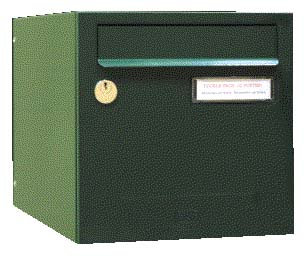
\includegraphics[height=1cm]{Fig-crypto/boite.jpg}}
      \end{picture}
    \end{center}
  \end{figure}

~


Clés d'Alice
\begin{itemize}
\item publique : \public{$n$} et \public{$e$}
\item privée : \prive{$d$}
\end{itemize}
%% Grand schéma 
%% Alice / Bob
%% $(n,e),d$

%% $m, x = m^d, m = x^e$
\end{frame}


%%%%%%%%%%%%%%%%%%%%%%%%%%%%%%%%%%%%%%%%%%%%%%%%%%%%%%%%%%%%%%%%
\section{Lemme de déchiffrement}

% \begin{frame}
% 
% \begin{lemme}
% Soit $d$ l'inverse de $e$ modulo $\varphi(n)$ avec $n=pq$.
% \mybox{Si \quad  $x \equiv m^e \pmod n$ \quad  alors \quad  $m \equiv x^d \pmod n$}
% \end{lemme}
% 
% \pause
% 
% \begin{proof}
% \begin{itemize}
%   \item 
%   \begin{itemize}
%     \item $d$ est l'inverse de $e$ modulo $\varphi(n)$
% \pause    
%     
%     \item $d \times e \equiv 1 \pmod {\varphi(n)}$
% \pause    
%     
%     \item il existe $k \in \Zz$ tel que $d \times e = 1 + k \times \varphi(n)$
%   \end{itemize}
%   
% \pause  
%   \item Petit théorème de Fermat amélioré
%   
% \pause  
%   \centerline{$m^{\varphi(n)} = m^{(p-1)(q-1)} \equiv 1 \pmod n$}
% 
% \pause  
%   \item Si $x \equiv m^e \pmod n$ alors
% \vspace*{-1ex} 
% $$
% \begin{array}{rl}
% x^d   \pause& \equiv (m^e)^d  \pause\equiv  m^{e\times d}  \pause\equiv m^{1+k \times \varphi(n)} \\
%       & \pause\equiv m \times m^{k \times \varphi(n)}  \pause\equiv m \times (m^{\varphi(n)})^k \\
%       & \pause\equiv m \times (1)^k \\
%       & \pause\equiv m \pmod {n}
% \end{array}$$
% \vspace*{-4ex}\qedhere
% \end{itemize}
% \end{proof}
% \end{frame}

% % % % % % % FR % % % % % %
\begin{frame}

\begin{lemme}
Soit $d$ l'inverse de $e$ modulo $\varphi(n)$ avec $n=p\times q$ \quad ($p\not= q$)
\mybox{Si \quad $x \equiv m^e \pmod n$ \quad alors \quad $m \equiv x^d \pmod n$}
\end{lemme}

\pause
\renewcommand{\qedsymbol}{}
\begin{proof}
\begin{itemize}
  \item 
  \begin{itemize}
    \item $d$ est l'inverse de $e$ modulo $\varphi(n)$
\pause    
    
    \item $d \times e \equiv 1 \pmod {\varphi(n)}$
\pause    
    
    \item il existe $k \in \Zz$ tel que $d \times e = 1 + k \times \varphi(n)$
  \end{itemize}
  
\pause  
  \item Petit théorème de Fermat amélioré
  
\pause  
  \centerline{si \quad $\pgcd(m,n)=1$ \quad alors \quad $m^{\varphi(n)} = m^{(p-1)(q-1)} \equiv 1 \pmod n$}

\pause  
  \item Si $\pgcd(m,n)=1$ alors modulo $n$ : %$x \equiv m^e \pmod n$ alors
\vspace*{-1ex} 
$$
\begin{array}{rl}
 (m^e)^d&  \pause\equiv m^{1+k \times \varphi(n)} \pause\equiv m \times m^{k \times \varphi(n)}  \\
      & \pause\equiv m \times (m^{\varphi(n)})^k  \pause\equiv m \times (1)^k \\
      & \pause\equiv m \pmod {n}
\end{array}$$
\vspace*{-6ex}%\qedhere
\end{itemize}
\end{proof}
\end{frame}

% % % % % % % FR % % % % % %

\begin{frame}

\begin{lemme}
Soit $d$ l'inverse de $e$ modulo $\varphi(n)$ avec $n=p\times q$ \quad ($p\not= q$)
\mybox{Si \quad $x \equiv m^e \pmod n$ \quad alors \quad $m \equiv x^d \pmod n$}
\end{lemme}



\begin{proof}
\begin{itemize}
  \item Si $\pgcd(m,n)\not=1$, par exemple $\pgcd(m,n)=p$ et $\pgcd(m,q)=1$, alors %$x \equiv m^e \pmod n$ alors
\pause 
\vspace*{-1ex} 
\begin{itemize}
\item modulo $p$ : $m   \equiv  0 $ \pause \quad  et \quad $(m^e)^d \equiv  0 $ \pause \quad donc \quad $(m^e)^d \equiv  m   \pmod{p}$
%\vspace*{-2ex}
\pause
\item modulo $q$ : $(m^e)^d  \equiv m \!\times\! (m^{\varphi(n)})^k \equiv m \!\times\! (m^{q-1})^{(p-1)k} \equiv m   \pmod{q}$
\pause 
\item $\pgcd(p,q)=1$
\vspace*{-4ex}

$$(m^e)^d  \equiv  m \pmod{n}$$
\qedhere
\end{itemize}

      
\end{itemize}
\end{proof}
\end{frame}



%%%%%%%%%%%%%%%%%%%%%%%%%%%%%%%%%%%%%%%%%%%%%%%%%%%%%%%%%%%%%%%%
\section{Algorithmes}

\begin{frame}[fragile]

Alice choisit \prive{$p$}, \prive{$q$} et \public{$e$}, calcule $\public{n}=\prive{p}\times \prive{q}$ et la clé secrète
\vspace*{-1ex}
{\small
\begin{algo}[rsa.py (1)]
\vspace*{-1ex}
\begin{lstlisting}
def cle_privee(p,q,e) :
    n = p * q
    phi = (p-1)*(q-1)    
    c,d,dd = euclide_etendu(e,phi)   # Pgcd et coeff de Bézout
    return(d % phi)                         # Bon représentant  
\end{lstlisting}  
\end{algo} 
}

\smallskip
\pause

Le chiffrement d'un message \prive{$m$} connaissant la clé publique $\public{n}$ et $\public{e}$
\vspace*{-1ex}
{\small
\begin{algo}[rsa.py (2)]
\vspace*{-1ex}
\begin{lstlisting}
def chiffrement_rsa(m,n,e):
    return pow(m,e,n)  
\end{lstlisting}  
\end{algo} 
}

\smallskip
\pause

Seule Alice peut déchiffrer le message \public{$x$}, à l'aide de sa clé privée \prive{$d$}
\vspace*{-1ex}
{\small
\begin{algo}[rsa.py (3)]
\vspace*{-1ex}
\begin{lstlisting}
def dechiffrement_rsa(x,n,d):
    return pow(x,d,n)  
\end{lstlisting}  
\end{algo} 
}
\end{frame}





\end{document}
